\chapter{灵犀一指}

	\section{引言}
		灵犀一指是陆小凤自创的一门武功。这种武功不需要任何兵器,只需徒手就可将敌人制服。

	\section{灵犀一指的起源}
		陆小凤年轻时热衷武学,在西域一代游历时突发灵感,创立了灵犀一指,如图\ref{lxfbook}所示。

		\begin{figure}
			\centering
			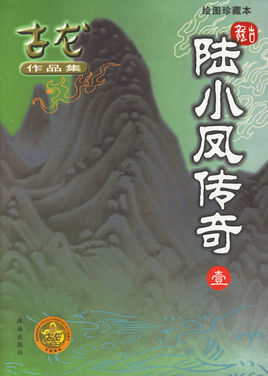
\includegraphics[width=.6\textwidth]{lxfbook.jpg}
			\caption{陆小凤传奇\label{lxfbook}}
		\end{figure}

	\section{灵犀一指要诀}
		灵犀一指是一种以柔制刚的武功,一般人很难领悟其中的精妙之处,因此很难学会。\cite{lxf:a}\citen{lxf:b} 实际上,它的要诀就是将内力汇聚在手指经脉之内,提高内力的密度,然后在瞬间释放出来,以致达到将敌人兵器折断的力道。如表\ref{lxfinsight}所示。

		\begin{table}
			\centering
			\caption{灵犀一指的要诀\label{lxfinsight}}
			\begin{tabular}{|c||c|}
				\hline
				步骤 & 操作\\
				\hline\hline
				1 &  气聚丹田\\
				\hline
				2 & 将丹田之气注入手指经脉\\
				\hline
				3 & 瞬间释放\\
				\hline
				4 & 将敌人制服\\
				\hline
			\end{tabular}
		\end{table}

		也可用算法表示,如算法\ref{algoinsight}所示。

		\begin{algorithm}
			\caption{\label{algoinsight}灵犀一指要诀}
			\begin{algorithmic}[1]
				\STATE 气聚丹田。
				\STATE 将丹田之气注入手指经脉。
				\STATE 瞬间释放。
				\STATE 将敌人制服。
			\end{algorithmic}
		\end{algorithm}

		也可用数学公式表示,如式\ref{mc2}所示。
		
		\begin{equation}
			E=mc^2
			\label{mc2}
		\end{equation}

	\section{本章小结}
		本章介绍了灵犀一指的要诀部分。
